\begin{frame}
  \begin{center}
    {\color{Maroon}\Huge Tackling a New Domain}
  \end{center}
\end{frame}

\begin{frame}{Tackling a New Domain}{Outline}
  \begin{enumerate}
  \item  Acoustic models for New Domains
    \begin{itemize}
    \item With no adaptation data
	\begin{itemize}
	  \item Robust Features
	  \item Feature compensation and test-time adaptation
          \item Multicondition training
	\end{itemize}
    \item With adaptation data
	\begin{itemize}
         \item Model adaptation
        \end{itemize}
    \end{itemize}
  \item  Language models for New Domains
    \begin{itemize}
    \item Commonly seen words in the new domain
    \item In-Domain data and other related data sources - Web data
    \end{itemize}
  \item Recipes for New Domains
  \end{enumerate}
\end{frame}

\begin{frame}{Acoustic Models in New Domains}{Robustness - Things Change}

\begin{itemize}
\item Background noise can increase or decrease.
\item  Channel can change.
\begin{itemize}
  \item Different microphone.
  \item Microphone placement.
  \item Location characteristics - Reverberation effect
\end{itemize}
\item Speaker characteristics vary.
\begin{itemize}
  \item Different vocal tract lengths (gender)
  \item Different speaking rates.
  \item Different accents
  \item Different age
\item There will always be speakers or conditions not represented well in the training data.
\end{itemize}
\item Heaven knows what else can happen.
\end{itemize}

\end{frame}


\begin{frame} {Acoustic models in ASR}{Recap:Probabilistic Model for Speech Recognition}

\begin{align*}
w^* & = \argmax_{w \in vocab} P(w | x, \theta) \\
       & = \argmax_{w \in vocab} \frac{P(x | w, \theta) P(w | \theta)} { P(x)} \\
       & = \argmax_{w \in vocab} {\color{red} P(x | w, \theta) }  P(w | \theta) \\
\end{align*}

\begin{itemize}
\item $w^*$  Best sequence of words
\item $x$ Sequence of acoustic vectors
\item $\theta$  Model Parameters
\end{itemize}
\end{frame}


\begin{frame}{Acoustic Models in New Domains}{What happens when things change?}
\setbeamercovered{invisible}

Recognition performance falls apart!

Why? \pause

Because the features on which the system was trained have changed. \pause

How do we mitigate the effects of such changes? What components of the system should we look at? \pause

The Acoustic Model: {\color{red} $P(x|W,\theta)$} and the features $x$ seem to be the most logical choices. So what can we do? 

\setbeamercovered{transparent}
\end{frame}

\begin{frame}{Acoustic Models in New Domains}{Robustness Strategies}

\setbeamercovered{invisible}

\pause

\begin{itemize}
\item {\bf Re-training:} Retrain system using the changed features. \pause
\item  {\bf Robust features:} Features $x$ that are independent of noise,
channel, speaker, etc. so $\theta$ does not have to be modified. \pause
  \begin{itemize}
     \item More an art than a science but requires little/no data. \pause
     \item Even with state-of-the-art neural networks that take the input audio as input to the first layer
  \end{itemize}
\item {\bf Modeling:} Explicit models for the effect the distortion (Noise, channel,speaker) has on speech recognition parameters $\theta' = f(\theta,D)$. \pause
  \begin{itemize}
  \item Works well when model fits, requires less data. \pause
  \end{itemize}
\item  {\bf Adaptation:} Update estimate of $\theta$ from new observations.  \pause
  \begin{itemize}
  \item Very powerful but often requires the most data $\theta' = f(D, p(O|W,\theta))$.
  \item Goal is to have an algorithm that adapts a large number of parameters with as little data from the new domain as possible
  \end{itemize}
  \end{itemize}

\setbeamercovered{transparent}
\end{frame}

\begin{frame}{General Retraining}

If the environment changes, retrain system from scratch in new environment.
  \begin{itemize}
  \item Very expensive - cannot collect hundreds of hours of data for each new environment.
  \item Also very expensive computationally and time-wise 
  \end{itemize}
Two strategies.
  \begin{itemize}
  \item Environment simulation.
  \item Multistyle Training.
  \end{itemize}


\end{frame}

\begin{frame}{Environment Simulation}

\begin{itemize}
\item Take training data 
\item Measure parameters of new environment 
\item Transform training data to match new environment 
\item Retrain system, hope for the best
\end{itemize}
\end{frame}


\begin{frame}{Multistyle Training}

\begin{itemize}
\item Take training data.
\item Corrupt/transform training data in various representative fashions (data augmentation)
\item Collect training data in a variety of representative environments.
\item Pool all such data together; retrain system.
\end{itemize}

\end{frame}


\begin{frame}{Issues with  Retraining}


Simplistic models of degradations
  \begin{itemize}
  \item E.g. telephony degradations more than just a different compression scheme based on the codec used
  \end{itemize}
Hard to anticipate every possibility.
  \begin{itemize}
  \item In high noise environment, person speaks louder with resultant
  effects on glottal waveform, speed, etc.
  \end{itemize}
Therefore other schemes - noise modeling and general forms of
  adaptation - are needed and sometimes used in tandem with these
  other schemes.


\end{frame}

\begin{frame}{Robust Features: Handling noise and channel variability}{Cepstral Mean Normalization}

Basic Idea: Assume all speech is linearly filtered but that the linear filter changes slowly with respect to speech (many seconds or minutes). \\

Effects from the channel or environment are usually modeled as \alert{additive or convolutive
distortions}

Given a set of cepstral vectors $O_{t}$ we can compute the mean:
\[ \bar{O} = \frac{1}{N}\sum_{t=1}^{N} O_t \]

\end{frame}

\begin{frame}{Robust Features (contd.)}


Linear channels have a convolutive effect - $y[n]$ = $x[n]*h[n]$, with
filter responses $h[n]$ that have a \alert{small time constants (less than 25ms)}. 

For frame index $k$
\begin{center}
$y_k[n]$ = $x_k[n]*h[n]$
\end{center}
Short-term cepstra (DCT of power spectrum) is modified by the linear channel,
\begin{center}
$Y_k(\omega)$ = $X_k(\omega)H(\omega)$\\
$\log(|Y_k(\omega)|^2)$ = $\log(|X_k(\omega)|^2)+log(|H(\omega)|^2)$\\
$C_y[k]$ = $C_x[k] + C_h$
\end{center}

\end{frame}

\begin{frame}{Robust Features (contd.)}
\begin{itemize}
\item To mitigate the effect of the linear  channel , In "Cepstral mean normalization'' we subtract the mean of a set of cepstral vectors from each vector individually
\[ \hat{O}_t = O_t-\bar{O} \]

\item When the speech signal is distorted with additive noise,  $y[n] = x[n] + q[n]$, uncorrelated with the speech signal, its effect can be mitigated by \alert{subtracting the estimate of the noise} from the signal.
Using a voice activity detector, the noise power spectral estimate is obtained as \alert{mean of the power spectrum in the non-speech region} and subtracted.
       \begin{center}
                $|\hat{X}_k(\omega)|^2 = |Y_k(\omega)|^2 - |\hat{Q}(\omega)|^2$
        \end{center}
\end{itemize}
\end{frame}

\begin{frame}{Robust Features (contd.)}
Reverberant speech is also modeled as a long-term convolution effect:
        \begin{center}
                $Y_k(\omega)$ = $X_k(\omega)R(\omega)$\\
                $\log(|Y_k(\omega)|)$ = $\log(|X_k(\omega)|)+log(|R(\omega)|)$
        \end{center}
        
Its effect is mitigated by subtracting the \alert{long-term} mean of $\log(|Y_k(\omega)|)$ 
\end{frame}
        
\begin{frame}{Issues}
\begin{itemize}
\item  Must be performed on both training and test data.
\item  Bad things happen if utterances are very short
\item  Bad things happen if there is a lot of variable length silence in the utterance
\end{itemize}

\end{frame}


\begin{frame} {Types of Acoustic Model Adaptation}
\begin{itemize}
\item {\color{blue} Supervised } vs. {\color{blue} Unsupervised:} Is correct transcription of utterance available at test time ?
\item {\color{blue} Batch} vs.{\color{blue}  Incremental adaptation:} Whole vs. small (time critical) portion of the test data is available (ideally suited for real-time systems)
\item What do we do if correct transcript is not available ?
\begin{itemize}
\item We obtain a first pass hypothesis using the best ASR system.
\item Use the above recognition result instead of the correct transcript.
\end{itemize}
\end{itemize}

\end{frame}

\begin{frame}{Handling speaker variability}

The goal is to fit acoustic model or features to the target speaker using the new acoustic adaptation data from the target speaker

\begin{itemize}

\item {\color{blue} Model-based - Feature-based:} \\
{\color{red} Adaptation} is the process of modifying the model to better fit the features  (eg. Maximum Likelihood Linear Regression)\\
{\color{red} Normalization}  is the process of transforming features to better fit  the model (eg. cepstral mean subtraction, feature based Maximum Likelihood Linear Regression)\\
\begin{itemize}
\item Can be done in a supervised or unsupervised manner
\item Can be implemented in batch or incremental mode
\end{itemize}
\end{itemize}
\end{frame}


\begin{frame}{But, we have a continuous stream of audio!}{Where are the speakers?}

{\color{blue} Properties:} Speaker identity, recording condition (e.g. background noise, telephone channel),
signal type (e.g. speech. music, noise, silence), and spoken content.

Segmentation and Clustering
\begin{itemize}
\item {\color{red} Segmentation:} Partitioning of the audio into homogeneous areas, ideally we should have one speaker/condition per segment.
\item {\color{red} Clustering:} Locating speakers and conditions involves the clustering of these segments into similar speakers/conditions.
\end{itemize}
\end{frame}

\begin{frame}{Processing the audio}
The performance of an ASR system is affected by:
\begin{itemize}
\item Segmentation affects speech recognition performance: speaker adaptation and speaker clustering assume one speaker per segment
\item Language model assumes sentence boundaries at the end of segments
\item Non-speech regions in the segment are often filled with noise and cause insertion errors
\item Overlapping speech is not recognized correctly, causing errors in the surrounding regions
\end{itemize}
\end{frame}

\begin{frame}{Segmenting the audio stream}
  
 Hypothesize segment boundaries:
 
\begin{itemize}
  \item  Input stream is modeled as Gaussian process in the cepstral domain.
  \item Feature vectors of one segment: drawn from multivariate Gaussian: $O_i^j := O_i \ldots O_j \sim \mathcal{N}(\mu, \Sigma)$ 

  \item For hypothesized segment boundary $t$ in $O_1^T$ decide between
    \begin{itemize}
 
    \item $O_1^T \in \mathcal{N}(\mu, \Sigma)$ and

    \item  $O_1^t \in \mathcal{N}(\mu_1, \Sigma_1)$ $O_{t+1}^T \in \mathcal{N}(\mu_2, \Sigma_2)$
    \end{itemize}
  \item Use difference of Bayesian Information Criterion values:
  \begin{align*}
    \Delta \mathrm{BIC}(t) &= \mathrm{BIC}(\mu, \Sigma, O_1^T) - \mathrm{BIC}(\mu_1, \Sigma_1, O_1^t) - \mathrm{BIC}(\mu_2, \Sigma_2, O_{t+1}^T) 
  \end{align*}
\end{itemize}

\end{frame}

\begin{frame}{Clustering of segmented audio}
\begin{itemize}
  \item  Group speech segments into clusters for adaptation.
  \item  Segments from same or similar speakers and conditions should be grouped together
   \item Greedy, bottom up clustering using acoustic features that merges segments
   \item Use Bayesian Information Criterion to control number of clusters that yields the best performance of the ASR system using one of the adaptation schemes mentioned in the next few slides
\end{itemize}

\end{frame}

\begin{frame}{Two classic Model Adaptation schemes for GMMs}{Maximum A Posteriori  - Basic Idea}

One way to achieve robustness is to take a fully trained HMM
system, a small amount of data from a new domain, and combine the
information from the old and new systems together. 

In Maximum A Posterior Estimation we assume there is some prior
probability distribution on $\theta$, $p(\theta)$ (the ASR system) and we try to
pick $\hat{\theta}$ to maximize the a posteriori probability of $\theta$ given the
observations (domain specific data):
\begin{eqnarray*}
\hat{\theta} & = & \argmax_{\theta} p(\theta|O_{1}^{N} ) \\
& = & \argmax_{\theta} \mathcal{L}(O_{1}^{N}|\theta) p(\theta)
\end{eqnarray*}

\end{frame}

\begin{frame}{Maximum a Posteriori Adaptation}{MAP}

\begin{enumerate}
\item Align adaptation data against a set of existing HMM models.
\item Collect counts $C_t(i,j)$, the fractional count (aka the posterior probability)  at time $t$ for being in mixture component $j$ of state $i$
\item Use this to estimate parameters of the adapted model
\end{enumerate}

For example,$\mu_{ik}$ is  the prior estimate for the mean of mixture
component $k$ for state $i$ from a previously trained HMM system. The adapted $\hat{\mu}_{ik}$:

\[ \hat{\mu}_{ik} =
  \frac{\tau_{ik}\mu_{ik}+\sum_{t=1}^{N}C_{t}(i,k)\O_t}{\tau_{ik}+\sum_{t}C_{t}(i,k)}
  \]
$\tau$ is a parameter that can be tuned to optimize performance on different test domains. 
\end{frame}

\begin{frame}{Maximum Likelihood Linear Regression - Basic Idea}{MLLR}

An alternate strategy is the popular MLLR adaptation scheme. In MAP, the different HMM Gaussians are free to move in any direction. \\
In Maximum Likelihood Linear Regression the means of the Gaussians are constrained to only move according to an affine transformation $Ax+b$.

\end{frame}

\begin{frame}{Feature transforms based on adaptation data}
\alert{Constrained/Feature MLLR}
        \begin{enumerate}
        \item Adaptation technique used in ASR to reduce the mismatch between acoustic
        features from a speaker and trained models \\
        \begin{center}
                $\hat{\mu} = A_c\mu - b_c$\\
                $\hat{\Sigma} = A_c \Sigma {A_c}^T$
        \end{center}
        \item Equivalent to transforming the features \\
        \begin{center}
                $\hat{o_t} = {A_c}^{-1}o_t + {A_c}^{-1}b_c$
        \end{center}
        \item Transformation parameters are estimated with EM to maximize the
        likelihood of the adaptation data
        \end{enumerate}
\end{frame}


\begin{frame} {Acoustic Model Adaptation with Neural Networks}

With the success of Neural Networks as a replacement for GMMs, all state-of-the-art ASR systems use a variant of deep neural networks.

Do the adaptation strategies for new domains still hold with neural networks? \pause

Stay tuned \ldots

\end{frame}

\begin{frame} {Acoustic Model Adaptation with Neural Networks}
\alert{Adaptation of neural network based acoustic models} - involves adapting a large number of parameters with a small amount of adaptation data. Recent advances include:
        \begin{itemize}
        \item \alert{Fine-tuning} - additional epochs of training of some or all layers of the network with the adaptation data alone (similar to new languages)
        \item \alert{Addition of additional layer} to perform a feature-space-like adaptation
        \item Use of a \alert{regularizer} to control the extent by which the weights move from the baseline model when trained with the in-domain audio
        \item Rely on \alert{feature adaptation} (fMLLR/ivectors) to serve as medium of adaptation and subsequently become the input to the neural network
        \end{itemize}
\end{frame}

\begin{frame} {Acoustic Model Adaptation with Neural Networks}

\alert{Weight decay based adaptation}: Similar to MAP adaptation, adapted network's weight updates are arrived at from using a  weighted combination of the updates from adaptation data and the baseline model
        \begin{center}
        $\Delta w_t = -\alpha{\nabla}_wE(w_t) - \beta(w_{t-1} - w_0)$ \\
        \vspace{1mm}
        \tiny{$\alpha$ - learning rate, $\beta$ - regularization parameter, $w_0$ - model parameters of the initial model}
        \end{center}
Useful for both \alert{speaker and domain adaptation}
\end{frame}

\begin{frame}{Weight decay based adaptation}{Performance of adapted ASR system}
\begin{columns}[T]
\column{2in}
\centering
{\color{orange}{Supervised Adaptation}}
\begin{center}
    \begin{tabular}{@{}cc@{}} \toprule
      {\bf Model} & {\bf WER\%} \\ \midrule
      Baseline SI CNN & 36.5 \\
      1 hr WD + sMBR & 30.9 \\
      2 hr WD + sMBR & 30.7  \\
      5 hr WD + sMBR & 30.1  \\
      10 hr WD + sMBR & 29.9  \\
      25 hr WD + sMBR & 28.2 \\ \bottomrule
    \end{tabular}
  \end{center}
\column{2in}
\centering
{\color{ForestGreen}{Unsupervised Adaptation}}
\begin{center}
    \begin{tabular}{@{}cc@{}} \toprule
      {\bf Model} & {\bf WER\%} \\ \midrule
      Baseline SI CNN & 36.5 \\
      2 hr WD + sMBR & 32.8 \\
      25 hr WD + sMBR & 31.4  \\
      75 hr WD + sMBR & 30.4  \\
      200 hr WD + sMBR & 30.3 \\ \bottomrule
    \end{tabular}
  \end{center}
\end{columns}
\end{frame}

\begin{frame} {How well do these techniques perform in unseen domains?}
{ASR in unseen domains - the ASPIRE challenge}

\begin{itemize}
\item Construct robust automatic speech recognition systems that \alert{without having access to matched training and
development data}.
\begin{itemize}
\item \alert{Training set}  - the Fisher conversational telephone training corpus (2,000 hours of transcribed telephone speech).
\item \alert{Test set} - Microphone speech recorded in noisy reverberant environments.
\end{itemize}
\item Techniques used by various sites:
\begin{itemize}
\item Data augmentation - Add up to 3000 hours of artificially created noisy reverberant speech
\item Neural network based speech enhancement - Train a denoising autoencoder to denoise speech signals
\item Robust Features and Feature adaptation - Robust features that compensate for artifacts
\item Robust acoustic models - models that use large context
\item Multiple systems and system combination - improvements of up to 15\% relative.
\end{itemize}
\end{itemize}
\end{frame}

\begin{frame}{ASR on unseen domains - the Aurora-4 challenge}

\begin{enumerate}
\item Aurora4 - A Medium vocabulary task, based on the Wall Street Journal corpus
\begin{enumerate}
\item Data collected from a primary Sennheiser microphone, and 18 other secondary microphones.
\item Six different noise types - airport, babble, car, restaurant, street traffic and train station, at 10-20 db SNR.
\end{enumerate}
\item Techniques used by various sites:
\begin{enumerate}
\item Multistyle Training
\item Denoising autoencoder to denoise speech signals
\item Denoising autoencoder together with noise estimates for input layer.
\item Joint training Neural network based frontend and backend acoustic models. 
\item Varying network topologies, such as the use of a linear activation layer to capture the dynamics of acoustic features for backend NN.
\end{enumerate}
\item State-of-the-art systems yield gains of up to 20\% relative on unseen microphone and noise conditions.
\end{enumerate}
\end{frame}


\begin{frame} {Language models for New Domains}{Does one size fit all?}
  \begin{center}
    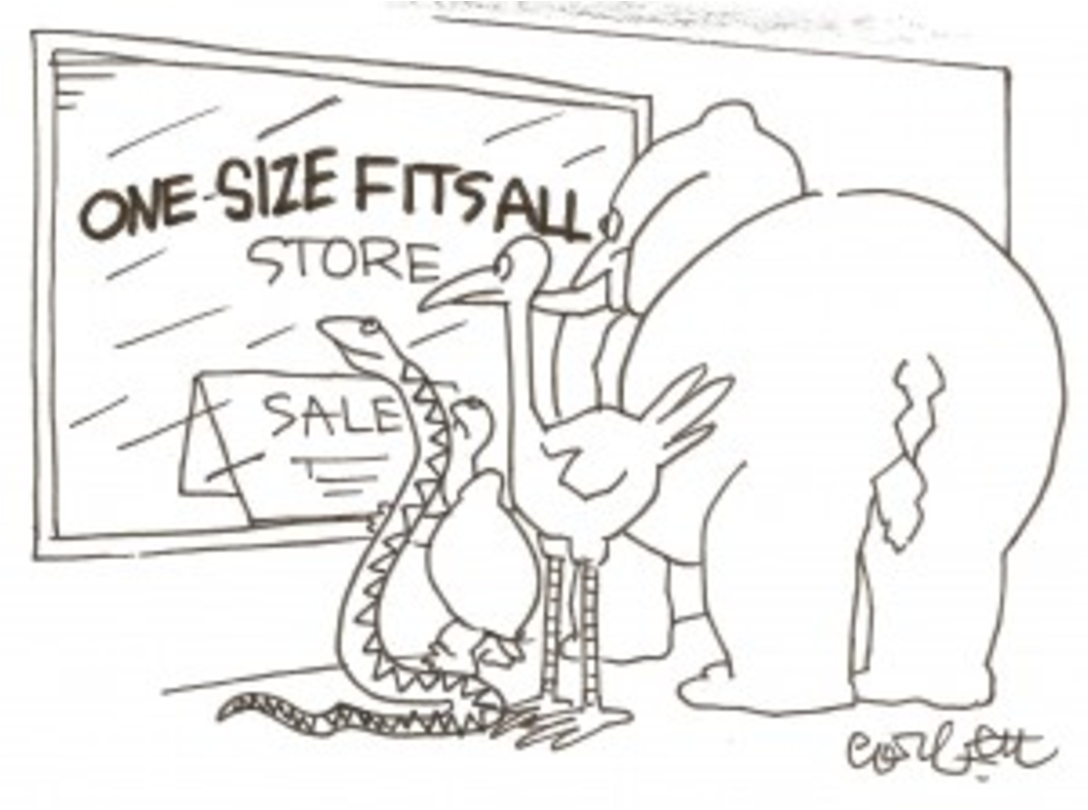
\includegraphics[width=77mm]{figures/onesize.pdf}
  \end{center}
\end{frame}

\begin{frame} {Language models for New Domains}{Does one size fit all?}

ASR systems are required to address a broad set of applications:
 \begin{itemize}
 \item  {\color{red}Conversation:} What is the best bar at this hotel?  What time is check out?
 \item  {\color{red}Chit Chat:} What are you doing? Are you a smart robot?
 \item  {\color{red}Question Answering:}What is the prognosis for Wernicke-Korsakoff Syndrome? What does Spondylolisthesis cause?
 \item  {\color{red} Analytics:} Call center customer support analysis for upselling, virtual agent, emotion analysis, etc.
 \item {\color{red}Transcription:} Broadcast news and sports captioning, podcast and YouTube transcriptions which address a wide variety of topics
 \end{itemize}

\end{frame}

\begin{frame}{Language models for New Domains}{Recap:Component blocks of ASR}
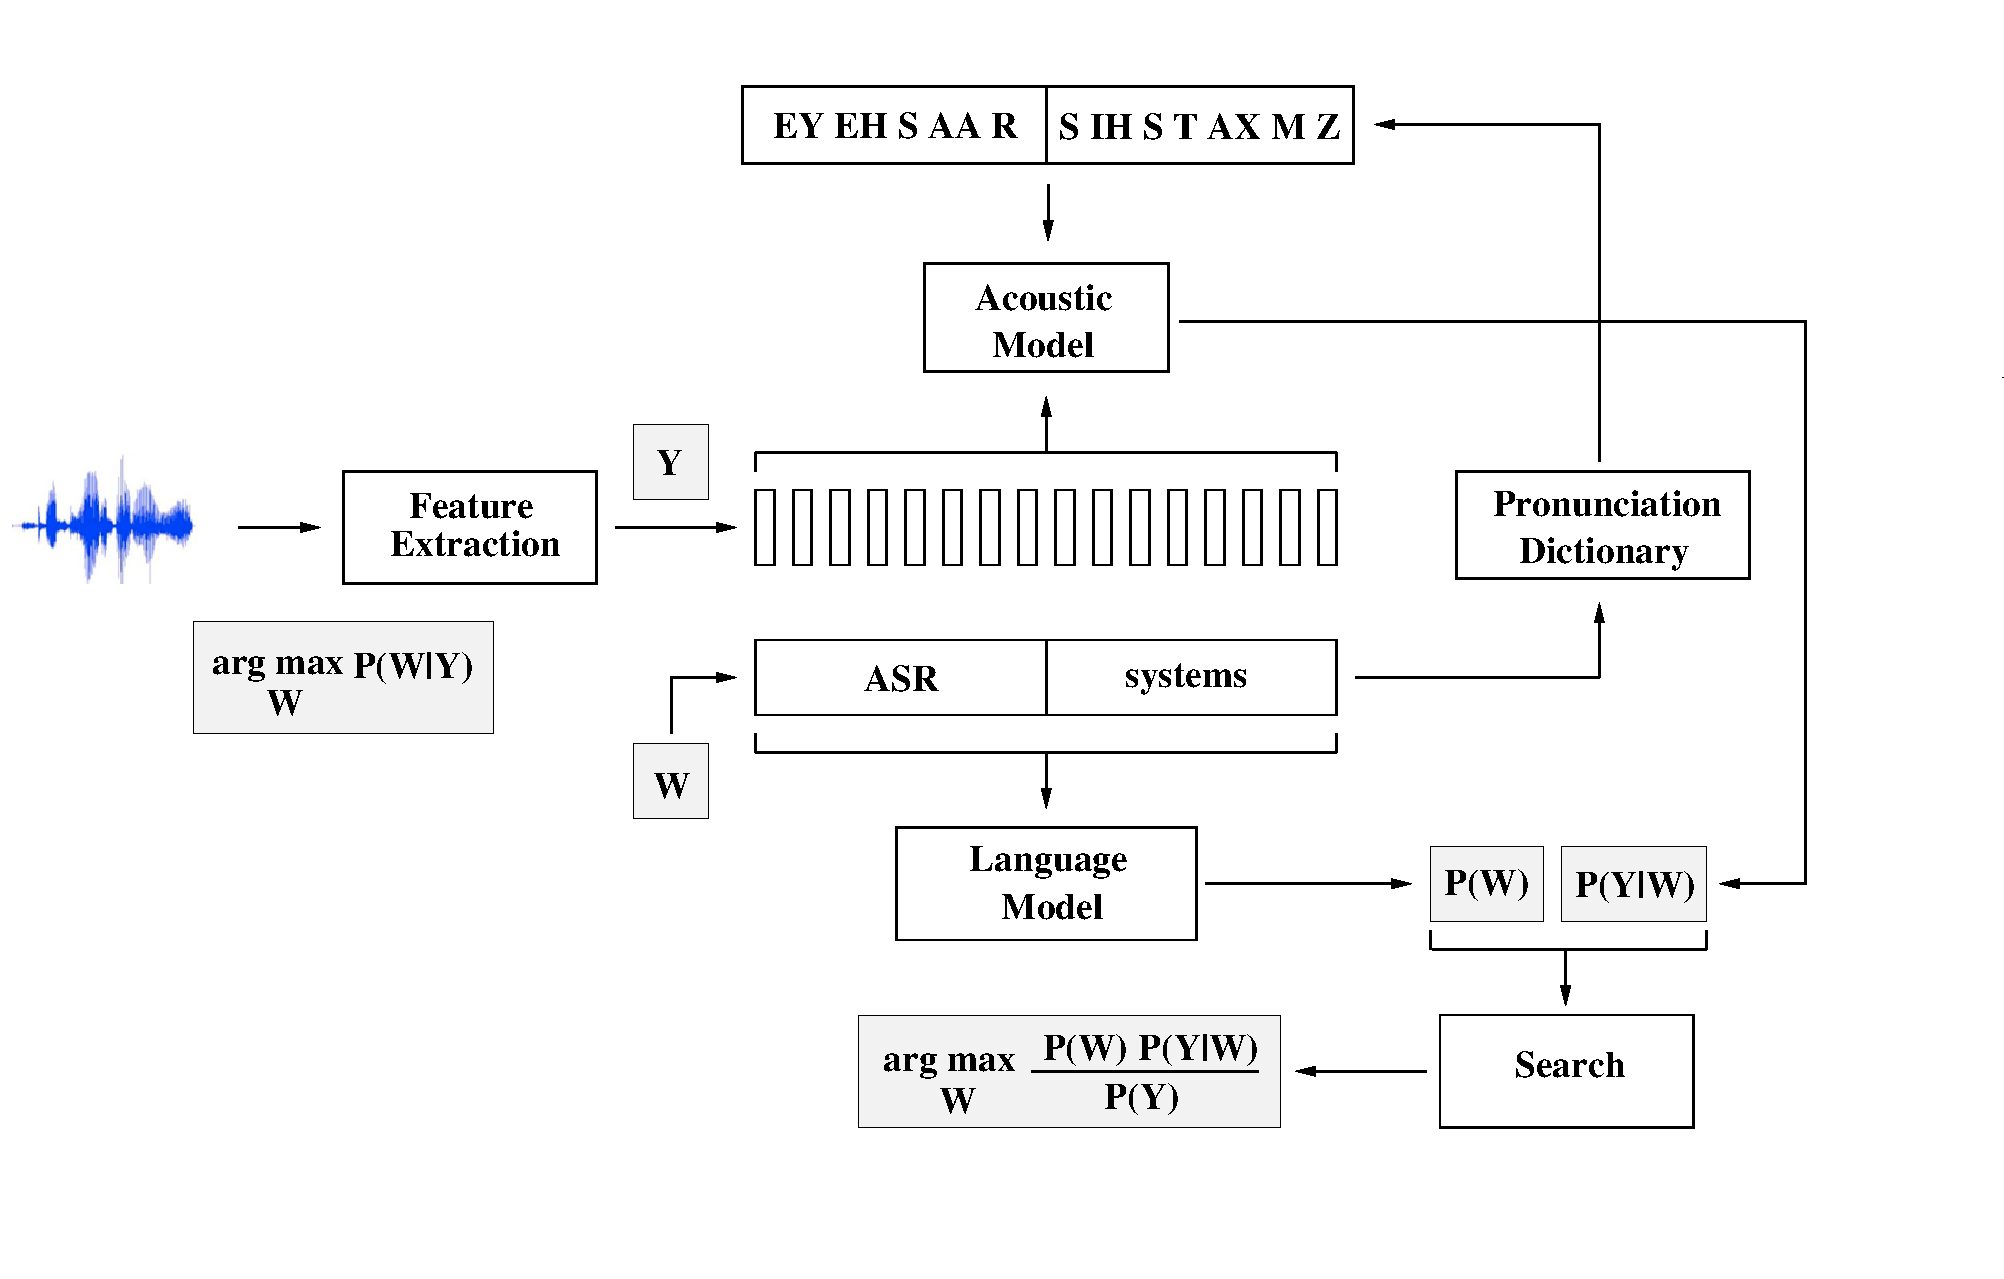
\includegraphics[height=77mm]{figures/ASR9}
\end{frame}

\begin{frame} {Language models in ASR}{Recap:Probabilistic Model for Speech Recognition}

\begin{align*}
w^* & = \argmax_{w \in vocab} P(w | x, \theta) \\
       & = \argmax_{w \in vocab} \frac{P(x | w, \theta) P(w | \theta)} { P(x)} \\
       & = \argmax_{w \in vocab} P(x | w, \theta)  { \color{red} P(w | \theta)} \\
\end{align*}

\begin{itemize}
\item $w^*$  Best sequence of words
\item $x$ Sequence of acoustic vectors
\item $\theta$  Model Parameters
\end{itemize}
\end{frame}

\begin{frame} {Language models in ASR}{Interpretation}

Specific to a \emph{domain}!!!

\begin{itemize}
\item Describes which word sequences are \emph{allowed}

\begin{itemize}
    \item Example: restricted domains like digit strings.
\end{itemize}

\item  Describe which word sequences are \emph{likely}
\begin{itemize}
   \item Example: unrestricted domains like web search.
   \item Example: {\it Britney Spears} vs {\it Brit knee spears}.
\end{itemize}

\item Analogy: multiple-choice test.
\begin{itemize}
    \item LM restricts choices given to acoustic model.
    \item The fewer choices, the better you do.
\end{itemize}

\end{itemize}

\end{frame}
    
\begin{frame}{Adapting to the new domain}{Strategies: New Words without context}

\begin{itemize}
\item Add new words (unigrams only with no context) relevant to the new domain ({\color{red} Out of Vocabulary} (OOV) words) to the base vocabulary of the ASR system
\item Pronunciations for these unigrams can be added or automatically generated

\begin{itemize}
\item Manual IPA pronunciation or
\item Automatically generate pronunciations from sample acoustics or
\item Automatically generate pronunciations from the graphemes/characters
\item Derive pronunciation from a sounds-like phrase (IEEE sounds like {\color{red} I triple E})
\end{itemize}

\item Modify  the pronunciation of new or existing words to suite the domain (for example, acronyms, such as, {\color{blue} HHonors} or {\color{blue} Hilton Honors})
\item  Add new words as unigrams with fixed probabilities to the {\color{blue} in-domain LM}
\end{itemize}
\end{frame}

\begin{frame}{Adapting to the new domain}{Strategies: New Words with context}

\begin{itemize}
\item Adapt the base LM using  corpora descriptive of the new-domain (text files), such as medical or legal texts with unique names and acronyms in the vocabulary
\item  In-domain text can be obtained either
\begin{itemize}
\item from existing files from the industry (product manuals, corporate FAQ websites, training manuals, etc.) or
\item by crawling the web or other data sources using relevant {\color{red} in-domain keywords} and obtaining large quantities of text to provide context for these new words
\end{itemize}
\item In-domain text can be augmented further by adding text obtained from words that are semantically similar to the in-domain keywords (for example, derived from neural word embeddings)
\begin{itemize}
\item {\color{blue} ``Speech''} is semantically similar to ``Address'', ``Statement'', ``Remarks'', ``Event ``, ``Ceremony''
\end{itemize}
\end{itemize}

\end{frame}

\begin{frame}{Adapting to the new domain}{Strategies: New Words with context}
\begin{itemize}
\item Derive new words that do not exist in the ASR system's vocabulary and add it to the lexicon 
\item Build an {\color{blue} in-domain LM} with the new in-domain corpora (with context for the new words) 
\end{itemize}

Interpolate the in-domain LM (statically or dynamically) with the base LM for use in the ASR system to obtain  the {\color{red} Domain Adapted LM}

\end{frame}

\begin{frame} {Domain Adaptation}{Overview}
  \begin{center}
    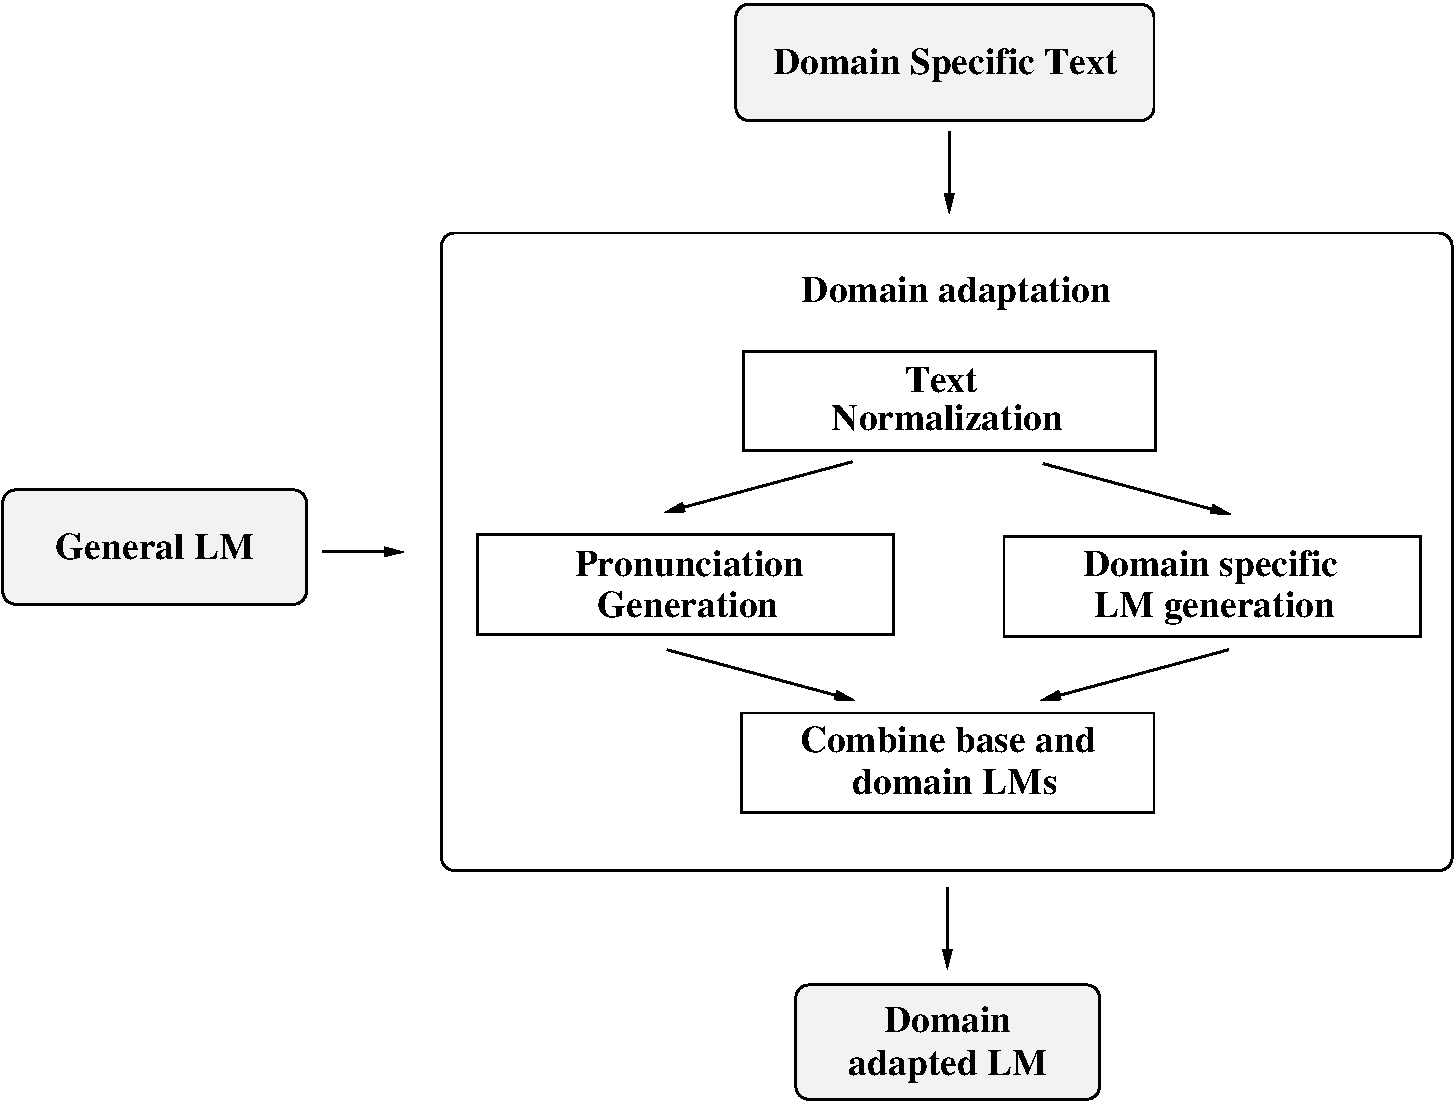
\includegraphics[height=65mm,width=90mm]{figures/DomainAdaptation.pdf}
  \end{center}
\end{frame}


\begin{frame}{Adapting to the new domain}{Challenges}

\begin{itemize}
\item Text normalization (90\% of language modeling is text normalization!)
\item LMs are usually very large with 100s of millions of n-grams) or complex, such as class-based exponential or neural network based models 
\item Can take very long to add just 10 new in-domain words and rebuild LMs! \pause
\end{itemize}
Solution is \ldots
\begin{itemize}
\item  Dynamically interpolate the new words and LM from the new domain
\item  Ensure the decoder is aware of new words in its look-ahead lists from both the base and the in-domain LMs
\end{itemize}

\end{frame}


\begin{frame}{What problem does a Domain Adapted LM solve?}{Examples}

\begin{itemize}
\item {\color{green} REF:  if i have had an {\color{purple} MRSA infection} or been told that i carry {\color{purple} MRSA} *  am i at high risk for developing  *  if i get seasonal influenza}
\item {\color{red} Base LM: if i have had an {\color{purple} IMMERSING FICTION }  or been told that i carry {\color{purple} IN MARSEILLE} I  am i at high risk for developing IT  if i get seasonal influenza}
\item {\color{blue} Domain Adapted LM::  if i have had an {\color{purple} MRSA infection} or been told that i carry {\color{purple} MRSA} I am i at high risk for developing IS  if i get seasonal influenza }
\end{itemize}
\end{frame}

\begin{frame}{Evaluating Language Models}{Did adaptation make the LM better?}

Best way: plug into ASR system, see how affects WER compared to base LM \\

Is there something cheaper that predicts WER well?
\begin{itemize}
\item {\color{red} {Perplexity} (PP) } of heldout or test data (needs only text).
\item Doesn't predict performance well \emph{across} LM types.
\item But does within single LM type!
\item Has theoretical significance.
\end{itemize}


\end{frame}


\begin{frame}{Performance of Domain Adapted LMs}{}
  Depending on the domain and the amount of in-domain text available, performance improvements in the range of 15-50\% relative can be seen.
  \vfill
  \centering
  \begin{tabular}{@{}lc@{}c@{}} \toprule
    {\bf Domain } &  {\bf Base LM } & {\bf Adapted LM } \\ 
    {\bf   } &  {\bf   \% WER} & {\bf \% WER } \\ \midrule
    Health care & 20.1 & 9.8 \\
    Call center&  26.6 & 22.7 \\ \bottomrule
  \end{tabular}
  \vfill
  \raggedright
  Results  presented are on in-house, customer data
\end{frame}


\begin{frame} {Suggested Combined Recipe for New Domains}
\begin{enumerate}
\item Obtain relevant in-domain text and include new words to the ASR system's lexicon
\item Using semantically similar or other relevant terms, derive additional text relevant to the domain
\item Build a domain adapted LM using all the above resource
\item Derive transcripts for the in-domain audio (supervised or unsupervised)
\item Use the domain adapted LM to obtain HMM state/character level alignments  of the in-domain audio (unsupervised) or the closed LM from reference transcripts for the same
\item Adapt the acoustic model using the audio, transcripts and the domain-adapted LM
\item You now have domain-dependent models that can be used in an ASR system
\end{enumerate}
\end{frame}

%\begin{frame} {Impact of Acoustic and Language Model Adapation on unseen call center data}
%{Weight Decay Adaptation and n-grams}
%Will add graph
%\end{frame}

